\documentclass[12pt,openright,oneside,a4paper,english,brazil]{abntex2}

% =====================================================================
% Pacotes e configurações básicas
% =====================================================================
\usepackage{lmodern}
\usepackage[T1]{fontenc}
\usepackage[utf8]{inputenc}
\usepackage{babel}
\usepackage{lastpage}
\usepackage{indentfirst}
\usepackage{microtype}
\usepackage{graphicx}
\usepackage{xcolor}
\usepackage{tikz}
\usepackage{stanli}
\usetikzlibrary{shapes.geometric, arrows.meta, positioning}
\usepackage{float}
\usepackage{listings}
\usepackage{amsmath}

% ------------------------------------------------------------------------
% CONFIGURAÇÃO DE LISTAGENS DE CÓDIGO - PACOTE LISTINGS
% ------------------------------------------------------------------------

% Paleta de cores (inspirada no VSCode claro)
\definecolor{codebg}{RGB}{248,248,248}
\definecolor{coderule}{RGB}{220,220,220}
\definecolor{codecomment}{RGB}{0,128,0}
\definecolor{codekeyword}{RGB}{0,0,180}
\definecolor{codestring}{RGB}{163,21,21}
\definecolor{codenumber}{RGB}{120,120,120}

% Estilo geral para códigos
\lstdefinestyle{defaultcode}{
    backgroundcolor=\color{codebg},
    basicstyle=\footnotesize\ttfamily,
    frame=single,
    rulecolor=\color{coderule},
    numbers=left,
    numberstyle=\tiny\color{codenumber},
    numbersep=7pt,
    tabsize=4,
    xleftmargin=2em,
    framexleftmargin=1.5em,
    breaklines=true,
    showstringspaces=false,
    captionpos=b,
    abovecaptionskip=5pt,
    belowcaptionskip=5pt,
    keywordstyle=\color{codekeyword}\bfseries,
    commentstyle=\color{codecomment}\itshape,
    stringstyle=\color{codestring},
    % Suporte a acentuação UTF-8
    literate={á}{{\'a}}1 {ã}{{\~a}}1 {â}{{\^a}}1 {à}{{\`a}}1 
             {é}{{\'e}}1 {ê}{{\^e}}1 {í}{{\'i}}1 {ó}{{\'o}}1 {ô}{{\^o}}1 {õ}{{\~o}}1 
             {ú}{{\'u}}1 {ç}{{\c{c}}}1 
             {Á}{{\'A}}1 {É}{{\'E}}1 {Í}{{\'I}}1 {Ó}{{\'O}}1 {Ú}{{\'U}}1,
}

% Aplica esse estilo globalmente
\lstset{style=defaultcode}

% Configurações de margens (ABNT: 3cm esquerda/superior, 2cm direita/inferior)
\setlrmarginsandblock{3cm}{2cm}{*}
\setulmarginsandblock{3cm}{2cm}{*}
\checkandfixthelayout

% Configuração de referências bibliográficas (BibLaTeX com estilo ABNT)
\usepackage{csquotes}
\usepackage[backend=biber,style=abnt]{biblatex}
\addbibresource{referencias.bib}

% =====================================================================
% Informações do trabalho (usadas na Capa, Folha de rosto, etc.)
% =====================================================================
\titulo{Abordagem VEM Híbrida Adaptativa com Deep Learning para Problemas Estruturais 2D com Estimativa de Incerteza}
\autor{Rafael Falcão Lacerda}
\local{São Paulo}
\data{2025}
\instituicao{
  Universidade de São Paulo\par
  Escola Politécnica\par
  Departamento de Engenharia de Estruturas e Geotécnica (PEF)
}
\tipotrabalho{Trabalho de Conclusão de Curso (Graduação em Engenharia Civil)}
\orientador{Prof. Dr. Rodrigo Provasi}
\preambulo{
  Trabalho de Conclusão de Curso apresentado ao Departamento de Engenharia de Estruturas e Geotécnica da Escola Politécnica da Universidade de São Paulo, como parte dos requisitos para a obtenção do título de Engenheiro Civil.\\
  \vspace*{0.5\onelineskip}
  \noindent Orientador: \imprimirorientador
}

% NOTA: O \hypersetup foi movido para depois do \begin{document}

\begin{document}

% =====================================================================
% CONFIGURAÇÃO DO HYPERREF - DEVE VIR AQUI, APÓS \begin{document}
% =====================================================================
\hypersetup{
    pdfauthor={\imprimirautor},
    pdftitle={\imprimirtitulo},
    pdfkeywords={TCC, Engenharia Civil, USP, ABNT},
    pdfcreator={LaTeX with abnTeX2},
    linkcolor=black,
    citecolor=black,
    filecolor=black,
    urlcolor=blue
}

% ============================================================
% Elementos Pré-textuais
% ============================================================

% Capa
\imprimircapa

% Folha de rosto (sem ficha catalográfica)
\imprimirfolhaderosto

% Resumo em Português
\setlength{\absparsep}{18pt}
\begin{resumo}
Este trabalho tem como objetivo aplicar e avaliar um framework híbrido que integra o Método dos Elementos Virtuais (VEM) com técnicas de Deep Learning para resolver problemas estruturais bidimensionais governados pela teoria da elasticidade linear, incorporando a quantificação de incertezas para aplicações em engenharia estrutural. A metodologia parte da utilização de um solver numérico baseado no VEM, já previamente desenvolvido e validado, para a geração de conjuntos de dados de alta fidelidade, contemplando diferentes configurações estruturais, propriedades materiais e condições de contorno. Esses dados alimentam uma rede neural profunda, também previamente implementada, capaz de aprender o mapeamento entre parâmetros geométricos/materiais e os campos de deslocamento e tensão resultantes.

A quantificação das incertezas epistemológicas é realizada por meio da técnica de Monte Carlo Dropout durante a inferência, gerando mapas de incerteza espacial que indicam regiões onde o modelo apresenta menor confiança. Estes mapas são utilizados como critério para a realização de refinamento adaptativo local da malha no VEM, retroalimentando o processo com dados mais precisos nas regiões críticas identificadas, dentro de um ciclo adaptativo iterativo. O desempenho do framework híbrido proposto é avaliado por meio da comparação de sua precisão e eficiência computacional com as soluções VEM puras (em malhas fixas), analisando aspectos de robustez e capacidade de generalização.
\vspace{1em}
\begin{center}
\textbf{Palavras-chave}: Método dos Elementos Virtuais; Deep Learning; Quantificação de Incertezas; Elasticidade Linear; Métodos Híbridos
\end{center}
\end{resumo}

% Abstract em inglês
\begin{resumo}[Abstract]
\begin{otherlanguage*}{english}
This work aims to apply and evaluate a hybrid framework that integrates the Virtual Element Method (VEM) with Deep Learning techniques to solve two-dimensional structural problems governed by linear elasticity theory, incorporating uncertainty quantification for structural engineering applications. The methodology starts from the use of a numerical solver based on VEM, already previously developed and validated, for the generation of high-fidelity datasets, covering different structural configurations, material properties, and boundary conditions. This data feeds a deep neural network, also previously implemented, capable of learning the mapping between geometric/material parameters and the resulting displacement and stress fields.

The quantification of epistemological uncertainties is performed using the Monte Carlo Dropout technique during inference, generating spatial uncertainty maps that indicate regions where the model exhibits lower confidence. These maps are used as the criterion for performing local adaptive mesh refinement (AMR) in the VEM, feeding the process back with more precise data in the critical regions identified, within an iterative adaptive cycle. The performance of the proposed hybrid framework is evaluated by comparing its accuracy and computational efficiency with pure VEM solutions (on fixed meshes), analyzing aspects of robustness and generalization capability.
\vspace{1em}
\begin{center}
\textbf{Keywords}: Virtual Element Method; Deep Learning; Uncertainty Quantification; Linear Elasticity; Hybrid Methods
\end{center}
\end{otherlanguage*}
\end{resumo}

% Sumário
\tableofcontents*

\textual

\chapter[Introdução]{Introdução}
\addcontentsline{toc}{chapter}{Introdução}

O presente trabalho propõe e avalia um framework híbrido que integra o Método dos Elementos Virtuais (VEM) e Deep Learning (DL) para a resolução de problemas estruturais bidimensionais, sob a teoria da elasticidade linear, incorporando a quantificação de incertezas. A metodologia utiliza um solver VEM existente e validado para gerar conjuntos de dados de alta fidelidade. Estes dados abrangem 
distintas configurações estruturais, propriedades de materiais e condições de contorno, servindo como base para o treinamento do modelo de DL.

Emprega-se uma rede neural profunda para aprender o mapeamento entre os parâmetros de entrada (geometria, materiais) e os campos de solução (deslocamentos e tensões). A quantificação da incerteza epistemológica, inerente ao modelo de DL, é realizada através da técnica de Monte Carlo Dropout. Esta abordagem permite a obtenção de mapas espaciais de incerteza durante a fase de inferência, os quais 
indicam as regiões onde as predições da rede neural possuem menor confiança.

Os mapas de incerteza constituem o critério central para o refinamento adaptativo da malha. O framework utiliza essa informação para direcionar novas análises VEM de maior fidelidade especificamente nas regiões críticas identificadas pela rede. Este ciclo adaptativo (inferência DL, quantificação de incerteza, refinamento VEM) é iterado até que a convergência da solução e a redução da incerteza 
atinjam os limiares predefinidos.

O desempenho da abordagem híbrida adaptativa será avaliado comparativamente, focando na precisão da solução e no custo computacional total, confrontando-a com a solução VEM pura em malhas fixas (grosseiras e refinadas). Espera-se que a integração da quantificação de incerteza viabilize a identificação eficiente das regiões que exigem refinamento, otimizando o processo de simulação e resultando 
em soluções estruturais mais confiáveis.

\chapter{Revisão Bibliográfica}

A análise computacional de problemas de elasticidade em engenharia estrutural tem apresentado avanços expressivos nas últimas décadas, impulsionada pelo desenvolvimento de métodos numéricos robustos e, mais recentemente, pela incorporação de técnicas de inteligência artificial. Esta revisão bibliográfica delineia essa trajetória, desde os métodos clássicos de formulação matemática até as 
abordagens híbridas contemporâneas que unem fundamentos físicos consolidados e capacidade de generalização baseada em aprendizado de máquina.

Inicialmente, são revisados os métodos numéricos que formam a base da análise estrutural moderna, com destaque para o Método dos Elementos Finitos (FEM) e sua extensão natural, o VEM. Em seguida, discutem-se os avanços e variações do VEM que ampliaram sua aplicabilidade a domínios com geometrias complexas e comportamento estrutural heterogêneo.

Posteriormente, são examinadas as contribuições recentes da inteligência artificial para a modelagem computacional em engenharia estrutural, com ênfase em redes neurais profundas e em técnicas que incorporam conhecimento físico em seu processo de treinamento. Analisa-se o potencial dessas abordagens para acelerar simulações e aprimorar a eficiência computacional, bem como suas limitações 
associadas à dependência de dados e à quantificação da incerteza.

A quantificação de incertezas emerge como um elemento central nas aplicações de aprendizado profundo em engenharia, dada a necessidade de avaliar a confiabilidade das predições obtidas por modelos estatísticos. Assim, são discutidos os principais métodos empregados para essa finalidade e sua relevância no contexto de modelos híbridos.

Por fim, a revisão apresenta os desenvolvimentos recentes em estratégias híbridas que integram métodos numéricos, como o VEM, e modelos de aprendizado profundo. Essas abordagens buscam explorar a complementaridade entre a precisão física dos métodos clássicos e a capacidade preditiva das redes neurais, constituindo um campo de pesquisa promissor para o avanço da análise estrutural adaptativa 
e eficiente.

\section{Métodos Numéricos Clássicos em Elasticidade}

\subsection{Método dos Elementos Finitos (FEM)}

O Método dos Elementos Finitos (FEM) consolidou-se, desde meados do século XX, como a principal ferramenta numérica para a solução de problemas de elasticidade linear em domínios bidimensionais e tridimensionais. A formulação clássica baseia-se na discretização do domínio contínuo em elementos de geometria simples — tipicamente triangulares ou quadrilaterais no caso bidimensional — sobre os 
quais são definidas funções de forma polinomiais contínuas por partes.

Essa abordagem permite a aproximação sistemática das equações diferenciais governantes por um sistema algébrico de equações lineares, cuja solução fornece os deslocamentos nodais aproximados. A robustez, versatilidade e rigor matemático do FEM contribuíram para sua ampla adoção em análise estrutural, transferência de calor, escoamentos e diversos outros campos da engenharia.

Entretanto, o método apresenta limitações quando aplicado a domínios com geometrias complexas ou descontinuidades internas. A geração de malhas de alta qualidade, requisito fundamental para a estabilidade e precisão das soluções, torna-se um processo oneroso em regiões com fronteiras curvas, fendas, inclusões ou interfaces irregulares. Além disso, o FEM tradicional enfrenta dificuldades em 
acoplar malhas de diferentes resoluções sem recorrer a refinamentos globais, e sua formulação padrão não lida naturalmente com elementos poligonais de forma arbitrária, o que restringe sua flexibilidade em discretizações não estruturadas.

Essas limitações motivaram o desenvolvimento de métodos numéricos alternativos que preservam as propriedades de consistência e convergência do FEM, mas oferecem maior liberdade geométrica e adaptabilidade — entre os quais se destaca o VEM.

\subsection{Método dos Elementos Virtuais (VEM)}

Nesse contexto, o VEM emergiu como uma extensão natural do Método dos Elementos Finitos, projetada para superar suas limitações geométricas e topológicas \cite{beirao2013}. O VEM permite o uso de malhas compostas por elementos poligonais arbitrários — incluindo formas não convexas e com número variável de lados —, preservando as propriedades fundamentais de 
consistência e convergência do FEM.

A principal característica do método é dispensar a formulação explícita das funções de forma no interior dos elementos. Em seu lugar, o VEM define um espaço de soluções virtuais que reproduz exatamente polinômios até uma determinada ordem e utiliza operadores de projeção polinomial para calcular os termos necessários à formulação variacional. A contribuição de estabilização é então introduzida 
para garantir a unicidade e a estabilidade da solução, fechando o sistema de equações \cite{beirao2013}. Essa estratégia permite que o método mantenha a exatidão na reprodução de campos constantes e lineares, analogamente ao FEM, mas com maior flexibilidade para lidar com geometrias complexas e malhas não estruturadas.

Estudos comparativos indicam que, em problemas de elasticidade linear, o VEM alcança taxas de convergência e precisão equivalentes às do FEM em malhas regulares, apresentando desempenho superior em domínios de geometria irregular \cite{mengolini2019}. Entre suas principais vantagens destacam-se a capacidade de empregar malhas poligonais grosseiras adaptadas à forma do domínio, evitando 
refinamentos globais desnecessários, e a possibilidade de acoplar regiões discretizadas com diferentes resoluções ou topologias de maneira natural e consistente — um desafio típico para o FEM clássico \cite{mengolini2019}.

\section{Avanços e Extensões no VEM}

Desde a sua origem, o Método dos Elementos Virtuais tem passado por aprimoramentos e extensões que ampliam seu campo de aplicação.

\subsection{Elementos de Ordem Arbitrária (p-VEM)}

Um dos avanços relevantes no desenvolvimento do VEM foi a formulação de elementos de ordem arbitrária, conhecidos como p-VEM. Essa extensão, análoga ao p-FEM, permite elevar a ordem polinomial das funções aproximadoras sem a necessidade de refinar a malha. Dessa forma, a precisão numérica pode ser aprimorada por meio do aumento do grau das funções de base, mantendo-se inalterada a discretização do domínio.

Estudos demonstraram que o VEM de alta ordem preserva as propriedades ótimas de convergência e, em diversas situações, supera o desempenho do FEM de mesma ordem, principalmente devido à flexibilidade na escolha das malhas e à capacidade de representar domínios com geometrias complexas sem comprometer a estabilidade numérica \cite{mengolini2019}.

\subsection{Aplicações a Problemas Não Lineares}

O VEM também demonstrou desempenho robusto em aplicações que envolvem comportamentos não lineares de materiais, incluindo regimes elastoplásticos. \textcite{beirao2015} apresentaram uma formulação do VEM para problemas elasto-inelásticos em malhas poligonais, evidenciando que o método pode incorporar modelos constitutivos complexos — como leis tensão–deformação não lineares — de maneira direta e modular (black-box), sem comprometer a estabilidade numérica ou a precisão da solução.

Esses resultados reforçam a versatilidade do VEM em análises estruturais além do regime elástico linear, abrangendo fenômenos de plasticidade, dano e fratura, ao mesmo tempo em que preserva as principais vantagens do método, como a flexibilidade geométrica e a consistência em malhas não estruturadas.

\subsection{Elementos Virtuais Curvilíneos}

Um avanço relevante na formulação do VEM foi a introdução dos elementos virtuais curvilíneos, que permitem representar com precisão fronteiras suaves em domínios delimitados por curvas \cite{artioli2021}. Nessa extensão, as arestas dos elementos podem acompanhar o contorno curvo da geometria, eliminando o erro geométrico associado à aproximação por segmentos retos.

A formulação curvilínea adapta o espaço de forma virtual de modo a incluir todos os movimentos rígidos — rotações e translações do corpo indeformável — superando limitações observadas em formulações anteriores do VEM, nas quais certas componentes lineares não eram representadas exatamente \cite{artioli2021}. Essa modificação assegura a consistência cinemática do modelo e amplia sua capacidade 
de reproduzir soluções físicas com maior fidelidade.

Estudos numéricos demonstraram que, para elementos de ordem superior, a representação exata da geometria de fronteira resulta em ganhos significativos de precisão em comparação à versão poligonal tradicional do método \cite{artioli2021}. Do ponto de vista computacional, a transição do VEM padrão para o VEM curvilíneo exige apenas ajustes pontuais na implementação — principalmente nos 
cálculos de integrais de elemento e nas funções de forma ao longo do bordo — mantendo-se a estrutura geral do método inalterada. Essa característica reforça a viabilidade prática da abordagem, que combina rigor geométrico e estabilidade numérica com baixo custo adicional de implementação.

\section{Inteligência Artificial na Solução de PDEs}

Paralelamente à evolução dos métodos numéricos tradicionais, como o FEM e o VEM, a última década tem sido marcada pelo avanço das técnicas de aprendizado profundo aplicadas à solução de equações diferenciais parciais (PDEs) em problemas de mecânica dos sólidos.

\subsection{Physics-Informed Neural Networks (PINNs)}

Entre as abordagens de aprendizado profundo aplicadas à modelagem física, destacam-se as Physics-Informed Neural Networks (PINNs), introduzidas por \textcite{raissi2019}. Essas redes neurais são treinadas de modo a satisfazer diretamente as equações diferenciais parciais (PDEs) que regem o comportamento do sistema físico. O termo “informed” reflete o fato de que o conhecimento físico é 
incorporado à função de perda (loss function), que penaliza desvios em relação às equações de equilíbrio e às condições de contorno. Assim, em um problema de elasticidade linear, por exemplo, a loss inclui o residual das equações de Navier–Cauchy em pontos internos do domínio, bem como a violação das condições de contorno em pontos de fronteira \cite{lu2021}.

A diferenciação automática, disponível em frameworks modernos de deep learning, permite que a rede calcule de forma exata as derivadas espaciais necessárias (como deformações e tensões), dispensando o uso de malhas ou integração numérica tradicional. Dessa forma, as PINNs caracterizam-se como métodos mesh-free, aplicáveis a geometrias complexas e a problemas inversos ou mal-postos, nos quais 
dados experimentais podem ser incorporados à função de perda juntamente com as leis físicas do sistema.

Apesar dessa flexibilidade, as PINNs apresentam limitações em termos de eficiência e convergência. Estudos indicam que, em problemas diretos bem-postos — isto é, quando se deseja apenas resolver a PDE com condições de contorno conhecidas —, métodos numéricos clássicos baseados em malha, como o FEM e o VEM, ainda superam as PINNs em robustez e desempenho 
computacional \cite{karniadakis2021, lu2021}. O treinamento de uma PINN é frequentemente custoso e sensível à escolha de hiperparâmetros, exigindo elevado poder de processamento, especialmente em domínios de maior dimensão ou com gradientes acentuados. Além disso, redes densas convencionais sofrem com o chamado viés espectral, que dificulta a representação de componentes de alta 
frequência da solução \cite{wang2021}.

Por outro lado, as PINNs têm se mostrado particularmente eficazes em problemas inversos e de identificação de parâmetros, como a estimação de propriedades de materiais a partir de observações limitadas de deslocamentos ou tensões. Nesses casos, a integração conjunta de dados e restrições físicas no treinamento proporciona vantagens significativas em relação aos métodos puramente 
numéricos \cite{karniadakis2021}.

Diversas extensões têm sido propostas para aprimorar o desempenho das PINNs, incluindo esquemas de amostragem residual adaptativa — que aumentam a densidade de pontos de colocation em regiões de maior erro \cite{lu2021} — e arquiteturas de rede especializadas, como as baseadas em transformadas de Fourier ou wavelets, capazes de mitigar o viés espectral. Ainda assim, as PINNs não 
substituem integralmente os métodos numéricos consolidados para a resolução direta de PDEs, mas constituem uma ferramenta complementar valiosa, sobretudo pela capacidade de incorporar conhecimento físico e dados observacionais em um mesmo modelo.

\subsection{Outras Estratégias de Deep Learning}

Além das PINNs, diversas outras estratégias de deep learning têm sido exploradas com o objetivo de resolver equações diferenciais parciais (PDEs) ou acelerar simulações numéricas complexas. Entre essas, destacam-se as redes generativas e os modelos de redução de dimensionalidade baseados em autoencoders.

As Generative Adversarial Networks (GANs) vêm sendo utilizadas para gerar campos sintéticos que reproduzem propriedades estatísticas ou físicas de sistemas reais. Por meio do treinamento adversarial entre gerador e discriminador, essas redes aprendem distribuições de probabilidade subjacentes e podem produzir realizações plausíveis de campos aleatórios de propriedades materiais, microestruturas 
ou mesmo aproximações não supervisionadas de soluções estacionárias. Essa capacidade de gerar amostras consistentes com restrições físicas torna as GANs úteis em contextos de incerteza e modelagem estocástica, reduzindo o custo de obtenção de dados numéricos de alta fidelidade.

Outra linha relevante é o uso de autoencoders profundos, redes neurais projetadas para comprimir e reconstruir dados de forma não supervisionada. Em mecânica estrutural, essas arquiteturas têm sido aplicadas para reduzir a dimensionalidade de problemas parametrizados, identificando um espaço latente de baixa dimensão capaz de representar, com boa fidelidade, padrões típicos de 
deslocamentos ou tensões em uma estrutura. Uma vez aprendido esse espaço reduzido, o decodificador da rede pode mapear parâmetros físicos de entrada — como propriedades do material, condições de contorno e carregamentos — diretamente para os coeficientes latentes correspondentes. Essa abordagem permite prever campos completos de deslocamento ou tensão de forma significativamente mais 
rápida que a resolução direta via FEM ou VEM, mantendo um nível de precisão controlado.

\textcite{liang2018}, por exemplo, apresentaram um surrogate model baseado em deep learning capaz de estimar distribuições de tensões em estruturas bidimensionais com alta precisão, aprendendo a relação entre configurações de carregamento e respostas estruturais a partir de dados obtidos por simulações de elementos finitos. Esse tipo de modelo substituto (surrogate) oferece ganhos 
expressivos em análises paramétricas e processos de otimização, pois, após o treinamento, fornece resultados quase instantâneos em comparação com as simulações completas.

Modelos dessa natureza — incluindo autoencoders variacionais, redes convolucionais e arquiteturas baseadas em transformadores — ampliam o conjunto de ferramentas computacionais disponíveis na engenharia estrutural. Ao combinar aprendizado estatístico e conhecimento físico, essas abordagens oferecem caminhos promissores para enfrentar a alta dimensionalidade, a não linearidade e o custo 
computacional de problemas complexos em mecânica dos sólidos.

\section{Quantificação de Incertezas em Modelos de Deep Learning}

\subsection{Métodos Bayesianos e Heurísticos}

A quantificação de incertezas (UQ) em redes neurais aplicadas à engenharia estrutural constitui um aspecto essencial para a avaliação da confiabilidade dos resultados obtidos por modelos de aprendizado profundo. Diferentemente de métodos numéricos tradicionais, como o FEM, que permitem a estimativa de erro por meio de análises de malha — por exemplo, via cálculo de erro a posteriori —, 
as redes neurais convencionais produzem apenas valores pontuais de previsão, sem fornecer uma medida direta de confiança associada a essas respostas.

Para suprir essa limitação, diversas abordagens baseadas em inferência Bayesiana e métodos heurísticos têm sido incorporadas a modelos de deep learning. \textcite{gal2016} introduziram o conceito de Monte Carlo Dropout, demonstrando que a manutenção do dropout (desligamento aleatório de neurônios) também durante a fase de inferência, com múltiplas passagens estocásticas pela rede, permite 
estimar a dispersão das predições como uma medida de incerteza epistemológica. Essa técnica interpreta o dropout como uma aproximação de inferência Bayesiana, em que os pesos da rede passam a representar distribuições aleatórias induzidas pelo processo de desligamento. Com custo computacional reduzido, o método fornece intervalos de confiança para as respostas preditas, possibilitando 
identificar regiões do domínio ou condições de carregamento em que o modelo apresenta menor confiança.

De forma análoga, o DropConnect — variação em que o desligamento ocorre nas conexões de pesos em vez das ativações dos neurônios — pode ser aplicado sob o mesmo princípio. \textcite{mobiny2019} mostraram que o Monte Carlo DropConnect produz estimativas de incerteza consistentes com a inferência Bayesiana variacional, sem aumentar significativamente o número de parâmetros ou o custo de 
processamento, tornando-o adequado para redes de maior profundidade.

Além dessas aproximações, estudos sobre redes neurais Bayesianas explícitas vêm sendo conduzidos há décadas, atribuindo distribuições de probabilidade diretamente aos pesos e realizando inferência via métodos como Variational Inference ou Markov Chain Monte Carlo \cite{blundell2015}. Embora apresentem rigor teórico superior e ofereçam quantificação de incerteza mais precisa, essas 
abordagens são computacionalmente custosas para redes de grande escala aplicadas a problemas de engenharia, o que limita sua utilização prática. Nesse contexto, métodos aproximados como o dropout ganham destaque por conciliarem simplicidade e eficiência.

Outra linha relevante é o uso de ensembles de redes neurais, nos quais múltiplos modelos independentes são treinados sob diferentes inicializações ou subconjuntos de dados. A combinação de suas predições fornece tanto uma média mais robusta quanto uma medida da dispersão entre os modelos, interpretada como incerteza aleatória do preditor \cite{lakshminarayanan2017}. Essa estratégia, 
embora mais custosa que o Monte Carlo Dropout, tende a melhorar a robustez global do modelo e a estabilidade das predições em domínios complexos.

\subsection{Importância da Quantificação de Incertezas em Engenharia Estrutural}

A confiabilidade das previsões geradas por modelos computacionais é um aspecto crítico em aplicações de engenharia estrutural, especialmente em contextos onde a segurança é fator determinante. Em análises envolvendo tensões e deslocamentos, não basta obter uma estimativa pontual — é essencial conhecer o grau de incerteza associado a essa previsão. A quantificação de incertezas, portanto, 
assume papel central, permitindo avaliar a confiabilidade dos resultados numéricos e das predições baseadas em aprendizado de máquina.

No caso de modelos de deep learning, a ausência de mecanismos explícitos para medir incerteza limita sua aplicabilidade em situações críticas, nas quais é necessário identificar regiões ou condições sob as quais o modelo apresenta menor confiança. A incorporação de técnicas de quantificação de incerteza em redes neurais possibilita não apenas avaliar a variabilidade das respostas previstas, 
mas também orientar estratégias de refinamento adaptativo e calibração de modelos híbridos. Dessa forma, torna-se viável adotar o aprendizado de máquina com maior segurança em aplicações estruturais, garantindo que suas previsões sejam interpretadas de forma criteriosa e compatível com os requisitos de confiabilidade exigidos pela engenharia.

\section{Métodos Híbridos: Integração de Deep Learning e Métodos Numéricos}

Os avanços recentes em métodos numéricos e em aprendizado profundo têm impulsionado o surgimento de abordagens híbridas que buscam combinar a precisão física dos primeiros com a capacidade de generalização dos segundos. Esses frameworks integram o deep learning a métodos clássicos, como o Método dos Elementos Finitos e o Método dos Elementos Virtuais, explorando as 
complementaridades entre ambos. De modo geral, o conhecimento físico e a estrutura matemática dos métodos numéricos são utilizados para orientar o treinamento da rede neural, enquanto o modelo de aprendizado atua como componente interno capaz de aproximar soluções, acelerar simulações ou reduzir custos computacionais.

No contexto brasileiro, destaca-se o estudo de \textcite{provasi2025}, que desenvolveu um framework híbrido para a análise de vigas de Euler–Bernoulli combinando VEM e redes neurais profundas. O trabalho demonstrou o potencial dessa integração para construir modelos substitutos fisicamente consistentes e computacionalmente eficientes, estabelecendo um marco relevante para a 
aplicação de técnicas híbridas na modelagem estrutural.

\subsection{Elementos Finitos Aprendidos por Deep Learning}

\textcite{jung2020} introduziram o conceito de deep learned finite elements, em que redes neurais são incorporadas à formulação dos elementos finitos para gerar diretamente as matrizes de deformação, responsáveis por relacionar deslocamentos nodais e deformações. Nessa abordagem, a rede substitui as funções de forma explícitas, aprendendo a reproduzir propriedades fundamentais de um 
elemento clássico, como a capacidade de representar movimentos de corpo rígido e campos de deformação constantes com exatidão. Os resultados demonstraram que esses elementos aprendidos podem atingir acurácia superior à de elementos polinomiais convencionais, além de apresentarem maior adaptabilidade para extensões a formulações de ordem mais elevada, tridimensionais ou não lineares, uma 
vez que a rede pode ser treinada para otimizar o desempenho do elemento em diferentes condições estruturais.

Em continuidade a essa linha de pesquisa, \textcite{jung2022} propuseram o self-updated finite element (SUFE), no qual um elemento finito de placa com quatro nós é enriquecido por um procedimento iterativo orientado por aprendizado profundo que ajusta sua rigidez a cada iteração para compensar erros de discretização. Nesse modelo, a rede neural estima direções de flexão ótimas dentro do 
elemento, minimizando efeitos indesejados como o shear locking. Após poucas iterações de atualização interna, o elemento alcança melhorias significativas de precisão sem necessidade de refinar a malha, mantendo desempenho consistente mesmo em discretizações grosseiras e distorcidas \cite{jung2022}. Esses estudos evidenciam o potencial do aprendizado profundo para automatizar e adaptar 
formulações de elementos finitos, aprimorando a eficiência e a acurácia das simulações estruturais sem modificar o princípio fundamental da discretização numérica.

\subsection{Deep Energy Method (DEM) e Outras Estratégias Variacionais}

Uma vertente relevante no avanço das abordagens baseadas em aprendizado profundo para a solução de equações diferenciais parciais é a formulação de métodos variacionais híbridos, como o \textit{Deep Energy Method} (DEM) proposto por \textcite{samaniego2020}. Nessa formulação, a rede neural substitui explicitamente a malha e as funções de forma, atuando como função de aproximação para os 
campos de deslocamento. O treinamento é conduzido pela minimização da energia potencial total do sistema, de acordo com o princípio variacional da mínima energia — equivalente às equações de equilíbrio em sistemas conservativos.

Com essa construção, o método garante que, ao final do processo de otimização, a rede satisfaça de forma implícita as equações de equilíbrio, obtidas como condição de estacionariedade da energia, e respeite as condições de contorno essenciais, impostas diretamente na arquitetura da rede. A principal consequência é uma formulação sem malha, potencialmente mais escalável e robusta para problemas 
de elasticidade não linear e domínios de geometria complexa.

\textcite{samaniego2020} demonstraram a aplicabilidade do DEM em problemas de hiperelasticidade finita bidimensionais e tridimensionais, alcançando precisão comparável à do Método dos Elementos Finitos (FEM), mas sem necessidade de remalhamento em grandes deformações. Extensões subsequentes do método \cite{nguyen2021} aprimoraram a integração numérica e o tratamento das condições de contorno, 
além de aplicar o DEM a problemas multifísicos. Apesar desses avanços, desafios permanecem, especialmente no tratamento robusto das fronteiras e na melhoria da estabilidade e da convergência do treinamento em redes de maior complexidade.

\subsection{Frameworks Híbridos e Perspectivas Futuras}

Em vez de substituir completamente os métodos clássicos, diversas pesquisas recentes têm explorado a combinação direta entre solvers numéricos e redes neurais em esquemas híbridos. \textcite{meethal2023} apresentaram uma estratégia na qual a rede neural atua como um modelo de substituição (\textit{surrogate model}) de alta fidelidade, incorporando, entretanto, as matrizes e operadores do 
FEM em sua função de perda durante o treinamento. Nessa formulação, as equações do FEM — após a discretização do domínio e a aplicação das condições de contorno — são utilizadas como termos estruturantes da função de perda, garantindo que o aprendizado da rede permaneça em conformidade com as leis físicas discretizadas (\textit{physics-conforming}) e que o 
problema de otimização seja bem-posto.

Esse modelo híbrido FEM–RNA, por se apoiar no problema discreto previamente condicionado, demonstrou elevada eficiência na utilização de dados e superou o desempenho de abordagens baseadas exclusivamente em PINNs, apresentando maior acurácia e estabilidade em aplicações estruturais \cite{meethal2023}. Além disso, ao manter o arcabouço do FEM na fase de inferência, o método permite estimar o 
erro de predição de forma quantificável e possibilita a integração de módulos de quantificação de incerteza em conjunto com o solver numérico.

De modo geral, essas formulações híbridas ilustram o estado atual da arte na interseção entre aprendizado profundo e métodos numéricos. Em vez de abordagens concorrentes, ambas podem atuar de maneira complementar: as redes neurais oferecem rapidez e adaptatividade na predição, enquanto métodos como FEM ou VEM asseguram fundamentação física e estabilidade numérica. Essa integração tem 
produzido resultados expressivos, mitigando limitações inerentes a cada paradigma — como a rigidez de malhas fixas nos métodos numéricos ou a ausência de garantias de convergência no aprendizado puro — e delineando uma nova geração de ferramentas computacionais em engenharia estrutural. Nesse contexto, o presente trabalho insere-se ao propor um framework adaptativo que combina o VEM com 
modelos de aprendizado profundo munidos de quantificação de incerteza, investigando o desempenho e a robustez dessa abordagem híbrida em comparação com métodos clássicos.

\chapter{Objetivos}

O objetivo geral deste trabalho é desenvolver e avaliar uma abordagem híbrida adaptativa que integra o Método dos Elementos Virtuais (VEM) e técnicas de aprendizado profundo (Deep Learning) para a resolução de problemas estruturais sob a teoria da elasticidade linear, incorporando a quantificação de incertezas como critério de refinamento de malha.

O trabalho busca combinar a precisão física do VEM, utilizado como gerador de dados de referência, com a eficiência de inferência das redes neurais profundas. O modelo híbrido proposto é concebido para identificar regiões da estrutura onde as predições apresentam maior incerteza, promovendo o refinamento seletivo da malha apenas onde necessário e reduzindo o custo computacional total.

Os objetivos específicos são:

\begin{itemize}
    \item \textbf{Empregar um solver VEM previamente validado} para a geração de bases de dados sintéticas de alta fidelidade, variando parâmetros físicos e geométricos da estrutura, a fim de representar diferentes regimes de comportamento mecânico.
    \item \textbf{Desenvolver e treinar uma rede neural profunda supervisionada}, capaz de aprender o mapeamento entre as propriedades materiais, geométricas e de carregamento da estrutura e o campo de deslocamentos correspondente obtido via VEM.
    \item \textbf{Incorporar técnicas de quantificação de incerteza} ao modelo de rede neural, utilizando inferência estocástica com Monte Carlo Dropout para estimar a confiança das previsões e gerar mapas de incerteza espacial.
    \item \textbf{Propor um esquema de refinamento adaptativo de malha} guiado pelos mapas de incerteza, de modo a direcionar novas simulações VEM apenas às regiões onde a rede neural apresenta maior variabilidade preditiva.
    \item \textbf{Avaliar o desempenho do framework híbrido proposto}, comparando sua precisão e eficiência computacional com o VEM em malhas fixas, analisando a capacidade do modelo de reduzir o erro global com menor custo de processamento.
\end{itemize}

Com esse conjunto de objetivos, o estudo visa demonstrar o potencial do uso de técnicas de aprendizado profundo como ferramenta auxiliar para acelerar análises estruturais baseadas em métodos numéricos, preservando a consistência física das soluções e introduzindo mecanismos de refinamento guiados por incerteza.

\chapter{Metodologia}

\section{Descrição Geral da Metodologia Proposta}

A metodologia adotada neste trabalho foi estruturada para desenvolver e avaliar um modelo híbrido que combina o Método dos Elementos Virtuais (VEM) com técnicas de Deep Learning, aplicado 
à análise de uma viga engastada-livre submetida a carregamento distribuído constante. O processo foi organizado em três etapas principais, conforme o fluxograma conceitual apresentado na 
Figura~\ref{fig:fluxo_metodologia}.

\begin{figure}[H]
    \centering
    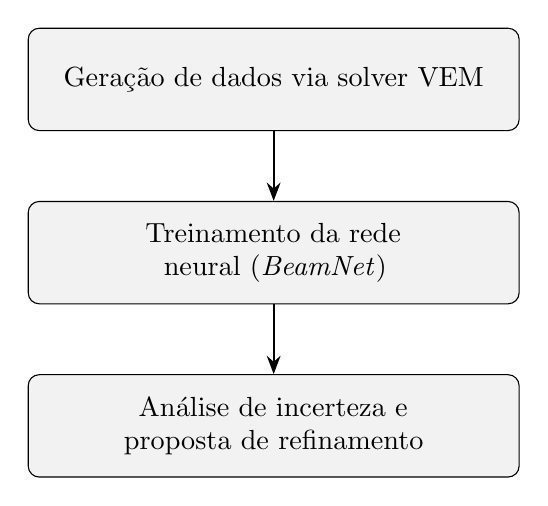
\begin{tikzpicture}[node distance=2.2cm]
        % --- estilos ---
        \tikzstyle{process} = [
            rectangle,
            rounded corners,
            minimum width=6cm,
            minimum height=1.3cm,
            text width=6cm,
            align=center,
            draw=black,
            fill=gray!10
        ]
        \tikzstyle{arrow} = [thick, ->, >=Stealth]

        % --- nós (etapas) ---
        \node (vem) [process] {Geração de dados via solver VEM};
        \node (nn) [process, below of=vem] {Treinamento da rede neural (\textit{BeamNet})};
        \node (uncert) [process, below of=nn] {Análise de incerteza e proposta de refinamento};

        % --- conexões ---
        \draw [arrow] (vem) -- (nn);
        \draw [arrow] (nn) -- (uncert);
    \end{tikzpicture}
    \caption{Fluxograma geral da metodologia adotada.}
    \label{fig:fluxo_metodologia}
\end{figure}

\textbf{Etapa 1 - Geração de dados por simulações VEM.} 
Inicialmente, um solver VEM previamente validado foi utilizado para simular o comportamento mecânico da viga sob diferentes combinações de parâmetros físicos. Nessa etapa, foram gerados 
conjuntos de dados contendo os deslocamentos e esforços internos correspondentes às condições de carregamento e propriedades geométricas e materiais da estrutura. O objetivo dessa fase foi 
obter um conjunto representativo de amostras que servisse de base para o treinamento e validação da rede neural.

\textbf{Etapa 2 - Treinamento da rede neural profunda com incerteza.} 
Com os dados obtidos, foi implementado e treinado um modelo de rede neural denominado \textit{BeamNet}, projetado para aproximar o campo de deslocamentos da viga a partir das variáveis 
de entrada. A rede foi treinada com o uso de \textit{Monte Carlo Dropout}, técnica que permite estimar a incerteza associada às previsões do modelo. Durante o treinamento, foram ajustados 
os parâmetros de aprendizado e monitoradas as métricas de erro de treino e validação, visando obter um modelo estável e generalizável.

\textbf{Etapa 3 - Análise dos diagramas de incerteza e proposta de refinamento.} 
Após o treinamento, foram gerados diagramas de incerteza a partir de múltiplas inferências estocásticas da rede neural. Esses diagramas permitem identificar regiões da estrutura em que o 
modelo apresenta maior variabilidade nas previsões. A partir dessa análise, propõe-se o uso dessas informações como critério para o refinamento adaptativo de malha no modelo VEM, de forma 
a direcionar o refinamento para as regiões onde a incerteza é mais elevada.

De forma geral, a metodologia busca combinar a precisão do VEM com a eficiência do \textit{Deep Learning}, utilizando a incerteza como guia para aprimorar o desempenho numérico de forma seletiva. Essa abordagem constitui a base do framework híbrido proposto, cuja estrutura modular permite futura extensão para problemas bidimensionais mais complexos.

%
\section{Geração dos Datasets via Solver VEM}

A geração do conjunto de dados utilizado para o treinamento e validação da rede neural foi realizada por meio de simulações numéricas conduzidas em um solver baseado no Método dos Elementos Virtuais (VEM) previamente desenvolvido e validado. O objetivo desse processo foi construir uma base de dados de alta fidelidade, composta por soluções numéricas de vigas engastadas-livres submetidas 
a carregamento distribuído constante, variando-se sistematicamente os parâmetros físicos relevantes.

O domínio estrutural considerado corresponde a uma viga de comprimento $L = 1{,}0\,\mathrm{m}$, discretizada em $40$ elementos unidimensionais igualmente espaçados. Para cada amostra, foram atribuídos valores distintos ao módulo de elasticidade $E$, ao momento de inércia $I$ e à intensidade do carregamento distribuído $q$, variando de acordo com intervalos definidos de modo a abranger 
diferentes regimes estruturais. As faixas de variação desses parâmetros estão apresentadas na Tabela~\ref{tab:dataset_ranges}.

\begin{table}[H]
\centering
\caption{Faixas de variação dos parâmetros utilizados na geração do dataset.}
\label{tab:dataset_ranges}
\begin{tabular}{lcc}
\hline
\textbf{Parâmetro} & \textbf{Mínimo} & \textbf{Máximo} \\ \hline
Módulo de elasticidade $E$ [GPa] & 50 & 250 \\
Momento de inércia $I$ [$\mathrm{m^4}$] & $1\times10^{-8}$ & $1\times10^{-6}$ \\
Carregamento distribuído $q$ [$\mathrm{N/m}$] & $-10^3$ & $-10^4$ \\ \hline
\end{tabular}
\end{table}

Os valores de $E$, $I$ e $q$ foram amostrados aleatoriamente dentro dos respectivos intervalos, assegurando diversidade e representatividade das condições estruturais simuladas. Para garantir a reprodutibilidade, utilizou-se uma semente fixa no processo de amostragem. No total, foram geradas $20\,000$ amostras independentes, cada uma correspondendo a uma combinação única de 
propriedades materiais e carregamento.

As condições de contorno adotadas replicam um engaste completo na extremidade esquerda da viga ($x = 0$), restringindo tanto o deslocamento vertical quanto a rotação, enquanto a extremidade oposta permanece livre. Para cada configuração amostrada, o solver VEM resolve o sistema estrutural, fornecendo como resposta o campo de deslocamentos ao longo da viga.

\begin{figure}[H]
    \centering
    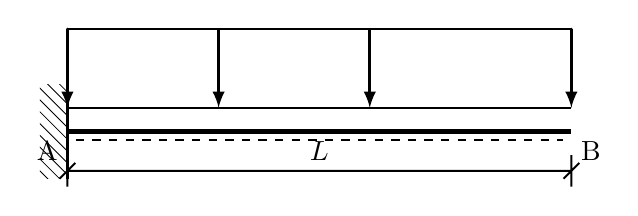
\begin{tikzpicture}
        % Escala (opcional - reduz o tamanho)
        \scaling{0.8};
        
        % Definir pontos
        \point{a}{0}{0};  % Ponto do engaste
        \point{b}{8}{0};  % Ponto final da viga
        
        % Desenhar a viga
        \beam{1}{a}{b};
        
        % Adicionar apoio engastado (tipo 3)
        \support{3}{a}[-90];
        
        % Adicionar carga distribuída (opcional)
        \lineload{2}{a}{b}[1][1][0.3];
        
        % Dimensões (opcional)
        \dimensioning{1}{a}{b}{-0.5}[$L$];
        
        % Notações (opcional)
        \notation{1}{a}{A}[below left];
        \notation{1}{b}{B}[below right];

    \end{tikzpicture}
    \caption{Viga engastada-livre sob carregamento distribuído constante $q_0$.}
    \label{fig:viga_engastada_livre}
\end{figure}

Com o intuito de normalizar as respostas e facilitar o treinamento da rede neural, os deslocamentos obtidos foram escalonados considerando um fator físico dependente dos parâmetros materiais, geométricos e de carregamento. Cada amostra gerada foi armazenada em formato tabular, contendo tanto os parâmetros de entrada quanto os deslocamentos resultantes nos nós da viga.

Ao final do processo, obteve-se uma base de dados estruturada, composta por $20\,000$ amostras sintéticas de alta fidelidade, cada uma representando a solução numérica de uma viga engastada-livre sob diferentes condições físicas. Essa base foi utilizada como referência supervisionada para o treinamento e validação do modelo de deep learning proposto, possibilitando a avaliação do 
desempenho do framework híbrido em cenários variados e realistas.

\section{Arquitetura e Treinamento da Rede Neural}
% (Explicação sobre a BeamNet, dropout, hiperparâmetros, etc.)

\subsection{Arquitetura da Rede Neural}

A arquitetura da rede neural foi projetada para aprender o mapeamento não linear entre os parâmetros físicos e geométricos da viga e o campo de deslocamentos resultante obtido pelo modelo numérico de referência. O objetivo é aproximar a relação entre as variáveis de entrada — módulo de elasticidade ($E$), momento de inércia ($I$), carregamento distribuído ($q$) e coordenadas 
espaciais — e a variável de saída, que corresponde ao deslocamento vertical escalonado ($w_\text{scaled}$) ao longo do comprimento da viga.

Os dados de entrada são previamente normalizados para garantir estabilidade numérica durante o treinamento. O modelo recebe, portanto, um vetor de dimensão $d_\text{in}=7$, que inclui parâmetros físicos, coordenadas nodais e termos auxiliares utilizados na parametrização do problema. A saída é um escalar que representa o deslocamento correspondente naquele ponto da estrutura.

A rede adotada segue a configuração de um Multi-Layer Perceptron (MLP) totalmente conectado, denominada \textit{BeamNet}, implementada no módulo \texttt{models.py}. Essa rede é composta por cinco camadas densas sequenciais com funções de ativação não lineares do tipo \texttt{Tanh}. As primeiras camadas possuem 512 neurônios, reduzindo progressivamente a dimensionalidade até a camada de 
saída, que contém um único neurônio de ativação linear. A função \texttt{Tanh} foi escolhida por apresentar melhor estabilidade durante o treinamento e capacidade de representar relações suaves entre variáveis contínuas. O código abaixo ilustra a estrutura simplificada da arquitetura:

\begin{lstlisting}[language=Python, caption={Estrutura da rede neural BeamNet.}]
class BeamNet(nn.Module):
    def __init__(self, input_dim=7, hidden_dim=512):
        super().__init__()
        self.net = nn.Sequential(
            nn.Linear(input_dim, hidden_dim),
            nn.Tanh(),
            nn.Linear(hidden_dim, hidden_dim),
            nn.Tanh(),
            nn.Linear(hidden_dim, hidden_dim // 2),
            nn.Tanh(),
            nn.Linear(hidden_dim // 2, hidden_dim // 4),
            nn.Tanh(),
            nn.Linear(hidden_dim // 4, 1)
        )
\end{lstlisting}

Com o objetivo de incluir a quantificação de incertezas nas previsões, foi desenvolvida uma variante denominada \textit{BeamNetDropout}, que insere camadas de \textit{Dropout} após cada camada densa intermediária. Durante o treinamento, o \textit{Dropout} atua como mecanismo de regularização, reduzindo o sobreajuste aos dados. Quando mantido ativo na fase de inferência, o mesmo recurso 
permite estimar incertezas epistemológicas por meio da técnica de \textit{Monte Carlo Dropout}. Essa abordagem será explorada na Seção~4.4. O trecho a seguir exemplifica a modificação introduzida:

\begin{lstlisting}[language=Python, caption={Variante BeamNetDropout com regularização e suporte à quantificação de incerteza.}]
class BeamNetDropout(nn.Module):
    def __init__(self, input_dim=7, hidden_dim=512, dropout_p=0.05):
        super().__init__()
        self.net = nn.Sequential(
            nn.Linear(input_dim, hidden_dim),
            nn.Tanh(),
            nn.Dropout(dropout_p),
            nn.Linear(hidden_dim, hidden_dim),
            nn.Tanh(),
            nn.Dropout(dropout_p),
            nn.Linear(hidden_dim, hidden_dim // 2),
            nn.Tanh(),
            nn.Dropout(dropout_p),
            nn.Linear(hidden_dim // 2, 1)
        )
\end{lstlisting}

Ambos os modelos foram implementados em \texttt{PyTorch} (versão 2.3) e projetados para treinamento em unidades de processamento gráfico (GPU), com suporte nativo ao backend \texttt{Metal (MPS)} no macOS. A arquitetura modular permite futura generalização para casos bidimensionais e integração com o framework híbrido VEM–Deep Learning em desenvolvimento.

\subsection{Treinamento da Rede Neural}

O processo de treinamento da rede neural teve como objetivo ajustar os parâmetros internos do modelo de modo que este aprendesse a reproduzir o comportamento estrutural representado nos dados obtidos via simulações VEM. Todo o procedimento foi implementado em \texttt{Python} utilizando o framework \texttt{PyTorch} (versão 2.3), e foi conduzido sobre a arquitetura \textit{BeamNetDropout}, 
que combina robustez numérica e capacidade de generalização por meio da regularização \textit{Dropout}. O treinamento foi executado em ambiente \texttt{macOS} com suporte a aceleração por GPU (\texttt{Metal Performance Shaders}).

O script principal de treinamento, denominado \texttt{train\_beamnet\_dropout.py}, foi estruturado em três componentes principais: (i) carregamento e normalização dos dados, (ii) definição do modelo, da função de perda e dos otimizadores, e (iii) execução dos ciclos de aprendizado e validação. O dataset supervisionado foi dividido automaticamente em subconjuntos de treino e validação com 
proporção de 90\% e 10\%, respectivamente, sendo processado em lotes (\textit{mini-batches}) de tamanho 512 por meio de \textit{DataLoaders}. Essa estratégia permite estabilizar o gradiente e otimizar o uso de memória durante o aprendizado.

A função de perda adotada foi o \textit{Mean Squared Error} (MSE), uma métrica clássica para problemas de regressão contínua, adequada à minimização das diferenças quadráticas entre deslocamentos previstos pela rede e valores de referência obtidos numericamente. O otimizador utilizado foi o \textit{Adam}, amplamente empregado em redes profundas por combinar adaptação dinâmica da taxa de 
aprendizado com bom desempenho em superfícies de perda não convexas. A taxa de aprendizado inicial foi definida como $1\times10^{-4}$, com ajuste automático via scheduler \textit{ReduceLROnPlateau}, que reduz o valor em 10\% após 80 épocas consecutivas sem melhoria no erro de validação.

Durante o treinamento, a rede percorreu 1200 épocas completas, e o desempenho foi monitorado tanto sobre o conjunto de treino quanto sobre o de validação. Em cada época, a perda média é calculada e registrada para análise posterior. Um sistema de \textit{early stopping} baseado na menor perda de validação foi implementado, de modo que o melhor modelo encontrado é salvo automaticamente 
em disco para evitar sobreajuste. O trecho a seguir resume a estrutura do loop de treinamento implementado:

\begin{lstlisting}[language=Python, caption={Loop de treinamento e validação da rede BeamNetDropout.}]
for epoch in range(EPOCHS):
    train_loss = train_one_epoch(model, train_loader, optimizer, criterion, device, epoch, EPOCHS)
    val_loss = validate(model, val_loader, criterion, device)
    scheduler.step(val_loss)

    if val_loss < best_val:
        best_val = val_loss
        torch.save(model.state_dict(), best_model_path)
\end{lstlisting}

Ao término do treinamento, são geradas automaticamente as curvas de aprendizado representando a evolução das perdas de treino e validação ao longo das épocas, salvas em formato \texttt{.png}. O modelo final é armazenado em formato \texttt{.pt}, incluindo os parâmetros da rede e os valores de normalização utilizados no pré-processamento dos dados. Essa prática garante reprodutibilidade 
e permite retomar a inferência diretamente em novas simulações sem necessidade de reescalar manualmente as variáveis.

O procedimento completo produz ainda um arquivo \texttt{summary.txt} contendo informações do experimento (hiperparâmetros, dataset utilizado, tempo total de execução e desempenho final). Essa estrutura modular foi adotada para facilitar comparações entre diferentes experimentos, mantendo rastreabilidade e padronização do processo de aprendizado. A Figura~\ref{fig:training_curve} (a ser 
incluída posteriormente) apresentará a curva de convergência característica do treinamento, evidenciando a estabilização das perdas após cerca de 1000 épocas.

De forma geral, o processo de treinamento mostrou-se estável e reprodutível, resultando em uma rede neural capaz de generalizar adequadamente as relações não lineares entre as propriedades estruturais e os deslocamentos previstos. Esse modelo treinado constitui o núcleo do componente de aprendizado do framework híbrido VEM–Deep Learning proposto, servindo como base para as análises de 
incerteza descritas na próxima seção.

\chapter{Resultados e Discussão}

\section{Desempenho do Treinamento da Rede Neural}

A Figura~\ref{fig:training_curve} apresenta a curva de aprendizado obtida durante o treinamento do modelo \textit{BeamNetDropout}. Observa-se uma rápida convergência das perdas de treino e validação nas primeiras 50 épocas, seguida de estabilização ao longo das demais iterações. O comportamento suave e consistente entre as duas curvas indica ausência de sobreajuste, evidenciando boa 
capacidade de generalização do modelo. A perda média quadrática (MSE) estabilizou em torno de $4\times10^{-1}$, representando erro relativo baixo nas predições de deslocamento escalonado.

\begin{figure}[H]
    \centering
    \includegraphics[width=0.8\textwidth]{../ml/experiments/dropout_sem_ponderacao_sem_scheduler/training_curve_dropout.png}
    \caption{Curva de aprendizado do modelo \textit{BeamNetDropout} durante o treinamento.}
    \label{fig:training_curve}
\end{figure}

\section{Análise de Incertezas na Viga Engastada-Livre}

Após o treinamento, o modelo foi avaliado em diferentes amostras do conjunto de validação. Para cada caso, foram realizadas 100 inferências estocásticas com \textit{Monte Carlo Dropout} ativo, obtendo-se o valor médio das predições e o desvio padrão associado. As Figuras~\ref{fig:uncertainty_0}--\ref{fig:uncertainty_75} apresentam os resultados para cinco amostras representativas.

Em todas as configurações, a rede neural reproduz adequadamente a tendência do deslocamento da viga obtida pelo solver VEM, com pequenas discrepâncias localizadas principalmente na extremidade livre, onde o gradiente de deslocamento é mais pronunciado. As faixas sombreadas representam os intervalos de confiança de $ \pm 2\sigma $, correspondentes à incerteza epistemológica estimada.

\begin{figure}[H]
    \centering
    \includegraphics[width=0.75\textwidth]{../ml/experiments/dropout_sem_ponderacao_sem_scheduler/uncertainty_sample_0000.png}
    \caption{Distribuição de deslocamentos e incertezas — amostra 0.}
    \label{fig:uncertainty_0}
\end{figure}

\begin{figure}[H]
    \centering
    \includegraphics[width=0.75\textwidth]{../ml/experiments/dropout_sem_ponderacao_sem_scheduler/uncertainty_sample_0010.png}
    \caption{Distribuição de deslocamentos e incertezas — amostra 10.}
    \label{fig:uncertainty_10}
\end{figure}

\begin{figure}[H]
    \centering
    \includegraphics[width=0.75\textwidth]{../ml/experiments/dropout_sem_ponderacao_sem_scheduler/uncertainty_sample_0025.png}
    \caption{Distribuição de deslocamentos e incertezas — amostra 25.}
    \label{fig:uncertainty_25}
\end{figure}

\begin{figure}[H]
    \centering
    \includegraphics[width=0.75\textwidth]{../ml/experiments/dropout_sem_ponderacao_sem_scheduler/uncertainty_sample_0050.png}
    \caption{Distribuição de deslocamentos e incertezas — amostra 50.}
    \label{fig:uncertainty_50}
\end{figure}

\begin{figure}[H]
    \centering
    \includegraphics[width=0.75\textwidth]{../ml/experiments/dropout_sem_ponderacao_sem_scheduler/uncertainty_sample_0075.png}
    \caption{Distribuição de deslocamentos e incertezas — amostra 75.}
    \label{fig:uncertainty_75}
\end{figure}

Nota-se que as regiões próximas ao engaste (\(x=0\)) apresentam menores níveis de incerteza, enquanto a extremidade livre exibe dispersões mais amplas, o que é fisicamente coerente com a maior sensibilidade estrutural nessa região. Esse comportamento valida a capacidade do \textit{Monte Carlo Dropout} em identificar zonas de maior incerteza preditiva, oferecendo um critério 
natural para o refinamento adaptativo de malha no modelo VEM.

\section{Síntese dos Resultados}

O modelo \textit{BeamNetDropout} apresentou convergência, estabilidade de aprendizado e boa generalização. As análises de incerteza demonstraram que a abordagem é capaz de capturar, de forma qualitativa e quantitativa, as regiões críticas da estrutura. Esses resultados confirmam a viabilidade do framework proposto e estabelecem a base para a etapa seguinte do trabalho, que 
consistirá na aplicação do método híbrido adaptativo em domínios bidimensionais.

\section{Perspectivas e Próximos Passos}

A continuidade do trabalho prevê três frentes principais de desenvolvimento:

\begin{itemize}
    \item \textbf{Refinamento da rede neural com dropout}: aprimorar o modelo \textit{BeamNetDropout} para reduzir os erros relativos em regiões de deslocamento de pequena magnitude, ajustando a regularização e os hiperparâmetros de treinamento.
    \item \textbf{Extensão para estruturas bidimensionais}: implementar e treinar uma nova arquitetura voltada à predição de campos de deslocamento em domínios 2D, com estudo de caso em uma chapa com furo central — exemplo clássico de concentração de tensões na análise de elementos finitos.
    \item \textbf{Integração adaptativa com o solver VEM}: desenvolver o módulo de refinamento de malha orientado por incerteza, no qual os mapas gerados pela rede neural guiarão localmente a rediscretização do domínio, formando o ciclo adaptativo completo do framework híbrido.
    \item \textbf{Correção e aprimoramento da visualização dos resultados}: ajustar a ordenação dos pontos nos gráficos de deslocamento gerados durante a inferência estocástica com \textit{Monte Carlo Dropout}. Os resultados apresentados refletem corretamente o comportamento físico esperado da viga e as incertezas associadas; entretanto, observou-se uma descontinuidade visual decorrente da ordenação incorreta de parte do vetor de coordenadas nodais no pós-processamento. A correção dessa etapa permitirá que as curvas sejam exibidas de forma contínua e monotônica, mantendo-se a coerência física e numérica já verificada nos dados.
\end{itemize}

Essas etapas consolidarão o modelo híbrido adaptativo proposto, permitindo sua aplicação a problemas estruturais mais complexos e a comparação sistemática entre as abordagens puramente numéricas e as híbridas.

% ============================================================
% Elementos Pós-textuais
% ============================================================
\postextual

\printbibliography[heading=bibintoc,title={Referências}]

\end{document}